This section treats the determination of the emissivity of the paint. To do so, we need the paint to be next to a surface of known emissivity. We use high emissivity tape with $\epsilon_\text{T} = \SI{0.95}{}$. In terms of equation \eqref{eq:powerTemp}, we can then write
\begin{align*}
	P_\text{P} &= \epsilon_\text{P}F(T_\text{P}) + (1-\epsilon_\text{P})F(T_\text{amb}) \text{\quad for the paint,} \\
	P_\text{T} &= \epsilon_\text{T}F(T_\text{T}) + (1-\epsilon_\text{T})F(T_\text{amb}) \text{\quad for the tape.}
\end{align*}
Assuming that both areas have the same real temperature because of their proximity and therefore emit the same amount of IR radiation, we set $P_\text{P}=P_\text{T}$. After rearranging, we obtain an equation for the emissivity of the paint
\begin{align}\label{eq:emissivity}
	\epsilon_\text{P} = \epsilon_\text{T}\frac{F(T_\text{T})-F(T_\text{amb})}{F(T_\text{P})-F(T_\text{amb})} \ .
\end{align}
%The surface temperatures $T_\text{P}, T_\text{T}$ are measure


In the following, we first describe the used set-up for measuring the emissivity of the paint and afterwards analyse the obtained data.
\subsection{Set-Up\label{sec:setup}}
As the petal will later be used at temperatures below \SI{0}{\degreeCelsius}, the thermal performance tests need to be adapted to low temperatures too. Therefore, we measure the emissivity of the paint on the cold side of a Peltier element. Actually, we use two Peltier elements next to each other covered by aluminium plates on the both sides. For simplicity, we shall refer to this combination of Peltier elements as 'the Peltier'. Figure \ref{fig:peltier} shows its cold side with the tape and paint. Additionally, we measure the surface temperature with pt100s. These values are a reference to the IR measurements and to control the Peltier. We calculate the emissivity with the IR data to guarantee comparability with the petal measurements which due to practical reasons cannot be done by pt100s all over the petal. \\


\begin{figure}[h!]
	\centering
	\includegraphics[width=0.8\textwidth]{img/PeltierCloseUp.png}
	\caption{Peltier element used for measuring the emissivity of the paint. We see the cold side with a taped and a painted area. There are also for thermocouples (type: pt100) which are named according to their position (e.g. TL means tape left). Additionally there is an IR camera measurement area next to each of the thermocouples.}
	\label{fig:peltier}
\end{figure}


\todo[noline]{Is the chiller also to reach lower temperatures?}
To ensure a low humidity to avoid ice formation, the Peltier sits in a cardboard box with dry air flushing that only leaves a hole for the camera lens. Furthermore to secure an optimal cooling of the Peltier, we cool its warm side using a chiller. \\


To gather the needed data, we run a current through the Peltier and wait some minutes until the pt100s and the voltage stabilise. Then we note the pt100 values as well as the temperature and radiance power for the four measurement areas as computed by the software. Additionally, we measure the ambient temperature and relative humidity in the box. We stop the measurement when the Peltier stops cooling efficiently (no stable minimum) or when ice forms on the Peltier. \\


We ran this routine three times trying to lower the humidity. Using humidity pearls worked well. Covering the inside walls of the cardboard box with acrylic glas did not lead to any improvement.
\subsection{Results}
Figure \ref{fig:emissivity} shows the results for the emissivity of the paint for all three runs. The values are all quite stable within the runs but vary a lot among them. We have no explanation for this yet.
\begin{figure}[h!]
	\centering
	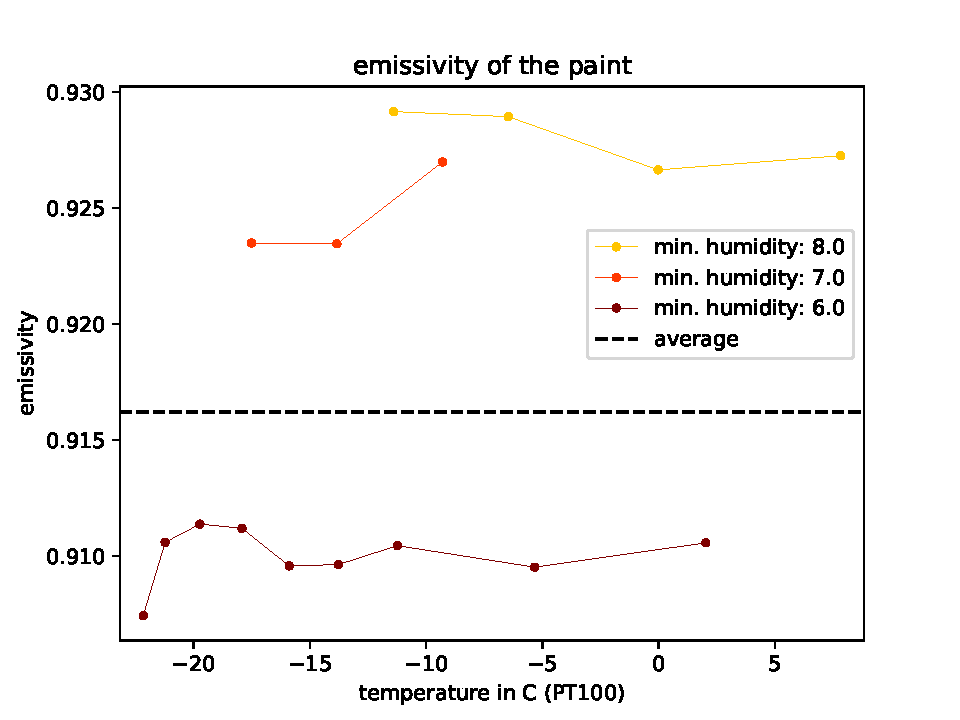
\includegraphics[width=0.7\textwidth]{img/emissivity.pdf}
	\caption{Emissivity values for the three different measurement runs with their absolute average.}
	\label{fig:emissivity}
\end{figure}


Figure \ref{fig:tempTemp} displays the difference in temperature between the pt100s and the corresponding IR measurement point taken at the respective emissivity value. For the tape values, this is mostly within the acceptable range of \SI{1}{\degreeCelsius} deviation. For the paint values the deviation reaches more than \SI{4}{\degreeCelsius}. Given the good result for the tape, we suspect our emissivity value of 0.920 to be wrong.
\begin{figure}[h!]
	\centering	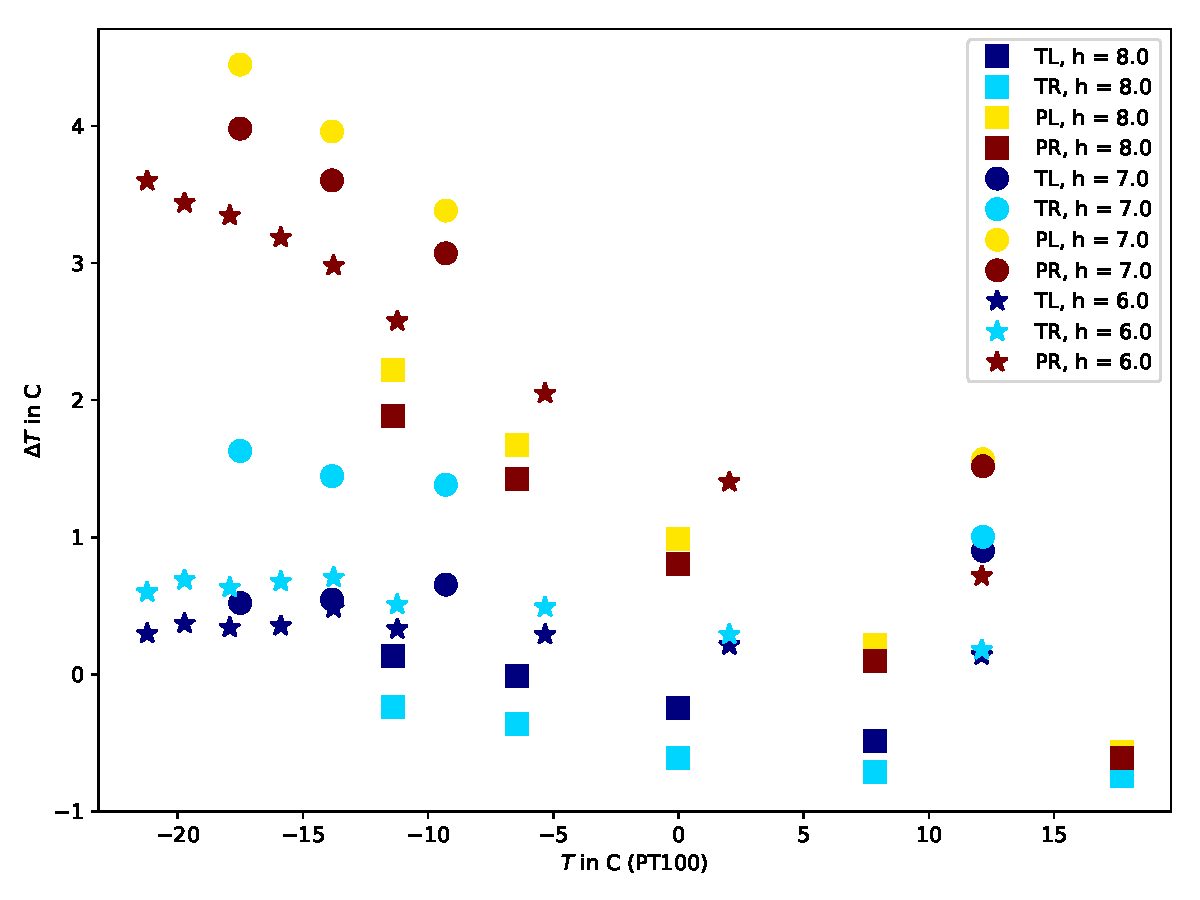
\includegraphics[width=0.8\textwidth]{img/temp_diff_oneplot.pdf}
	\caption{Temperature difference $\Delta T$ for all available data points in the three different measurement runs. For the tape the emissivity is set to \SI{0.95}{}, for the paint it is  \SI{0.92}{}.}
	\label{fig:tempTemp}
\end{figure}